\documentclass{beamer}
%\documentclass[xcolor=dvipsnames]{beamer}
\usepackage[spanish]{babel}
\usepackage[utf8]{inputenc}
\usepackage{graphicx}
\usepackage{latexsym}

\newcommand{\beamer}{\textsc{beamer}}
\newtheorem{definicion}{Definición}
\newtheorem{ejemplo}{Ejemplo}

%%%%%%%%%%%%%%%%%%%%%%%%%%%%%%%%%%%%%%%%%%%%%%%%%%%%%%%%%%%%%%%%%%%%%%%%%%%%%%%
\title[Trabajo de Fin de Grado]{Sistemas y Tecnologías Web\\
Aplicación para la elaboración y despliegue de cuestionarios}

\author[Juan José Labrador González] {
Autor: Juan José Labrador González \\
Director: Casiano Rodríguez León
}

\institute[ULL]{Escuela Superior de Ingeniería y Tecnología \\
                Departamento de Ingeniería Informática y de Sistemas \\
                Universidad de La Laguna}
\date[24-07-2014]{24 de Julio de 2014}
%%%%%%%%%%%%%%%%%%%%%%%%%%%%%%%%%%%%%%%%%%%%%%%%%%%%%%%%%%%%%%%%%%%%%%%%%%%%%%%

%\usetheme{Berlin}
\usetheme{Madrid}

%%%%%%%%%%%%%%%%%%%%%%%%%%%%%%%%%%%%%%%%%%%%%%%%%%%%%%%%%%%%%%%%%%%%%%%%%%%%%%%
\definecolor{pantone254}{RGB}{122,59,122}
\definecolor{pantone3015}{RGB}{0,88,147}
\definecolor{pantone432}{RGB}{56,61,66}
\setbeamercolor*{palette primary}{use=structure,fg=white,bg=pantone254}
\setbeamercolor*{palette secondary}{use=structure,fg=white,bg=pantone3015}
\setbeamercolor*{palette tertiary}{use=structure,fg=white,bg=pantone432}
\setbeamercolor*{palette sidebar primary}{use=structure,fg=pantone254}
\setbeamercolor*{palette sidebar tertiary}{use=structure,fg=pantone3015}
\setbeamercolor*{block title}{bg=pantone3015,fg=white}
\setbeamercolor*{alerted text}{fg=pantone432}
\setbeamercolor*{item projected}{fg=pantone254}
\setbeamercolor*{section in toc shaded}{use=structure,fg=structure.fg}
\setbeamercolor*{section in toc}{fg=pantone3015}
\setbeamercolor*{subsection in toc shaded}{fg=pantone3015}
\setbeamercolor*{subsection in toc}{fg=pantone432}

%%%%%%%%%%%%%%%%%%%%%%%%%%%%%%%%%%%%%%%%%%%%%%%%%%%%%%%%%%%%%%%%%%%%%%%%%%%%%%%
\begin{document}
  
%++++++++++++++++++++++++++++++++++++++++++++++++++++++++++++++++++++++++++++++  
\begin{frame}

  
\includegraphics[width=0.15\textwidth]{img/ullesc.eps}
  \hspace*{7.5cm}
  \includegraphics[width=0.16\textwidth]{img/etsii.eps}
  \titlepage

\end{frame}
%++++++++++++++++++++++++++++++++++++++++++++++++++++++++++++++++++++++++++++++  

%++++++++++++++++++++++++++++++++++++++++++++++++++++++++++++++++++++++++++++++  
\begin{frame}
  \frametitle{Índice}  
  \tableofcontents
\end{frame}
%++++++++++++++++++++++++++++++++++++++++++++++++++++++++++++++++++++++++++++++  

\section{Introducción}
\begin{frame}[allowframebreaks,fragile]
  \frametitle{Introducción}
  
  \begin{center}
    Este Trabajo de Fin de Grado consistió en la extensión de un Lenguaje de Dominio Específico ({\bfseries DSL}) que permite:
    \begin{itemize}
       \item La generación de cuestionarios autoevaluables para entrenamiento del alumnado.
       \item La generación de aplicaciones correctoras de exámenes provistas de lo necesario para su despliegue y puesta en funcionamiento.
    \end{itemize}
  \end{center}
  \framebreak
  %+++++++++++++++++++++++++++++++++++++++++++++++++++++++++++++++++++++++++++++++++++++++++++++++++++++++++++++++++++++++++++++++++++++++++++
  
  \begin{itemize}
    \item Fruto del estudio e investigación del estado del arte, se encontró un repositorio en GitHub con una gema de {\bfseries Ruby} denominada 
    \href{http://github.com/saasbook/ruql}{'RuQL'}:
    \begin{itemize}
      \item RuQL: Ruby-based Quiz Generator and DSL.
      \item Implementaba un DSL para hacer cuestionarios en diversos formatos usando distintos \textit{renderers}:
      \begin{enumerate}
        \item \textit{EdX}.
        \item \textit{AutoQCM} - AMC (\textit{Auto Multiple Choice}).
        \item \textit{Html5}.
      \end{enumerate}
      \item Los tipos de preguntas soportados por RuQL en ese momento eran: 
      \begin{itemize}
        \item De completar.
        \item De tipo test (respuesta única y multirrespuesta).
      \end{itemize}
    \end{itemize}
  \end{itemize}
  \framebreak
  %+++++++++++++++++++++++++++++++++++++++++++++++++++++++++++++++++++++++++++++++++++++++++++++++++++++++++++++++++++++++++++++++++++++++++++
  
  \begin{itemize}
    \item El creador de esta gema es \href{http://www.armandofox.com/geek}{{\bfseries Armando Fox}}, profesor del 
    \href{http://www.cs.berkeley.edu/}{Departamento de Ingeniería Informática y Eléctrica} de la 
    \href{http://www.berkeley.edu/}{{\bfseries Universidad de Berkeley}}, California (EEUU).
  \end{itemize}
  \begin{center}
    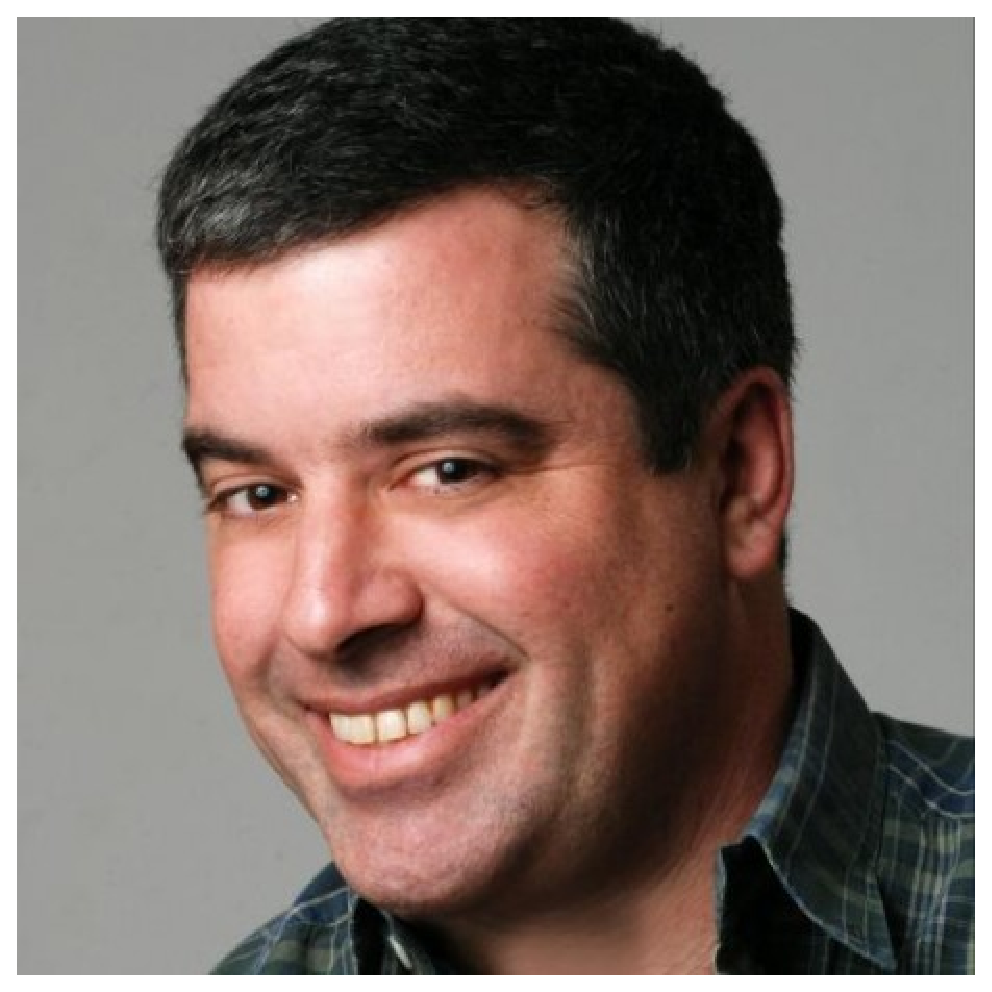
\includegraphics[width=0.2\textwidth]{img/armando.eps}
    \hspace*{0.8cm}
    
\includegraphics[width=0.2\textwidth]{img/Berkeley.eps}
    \hspace*{0.5cm}
    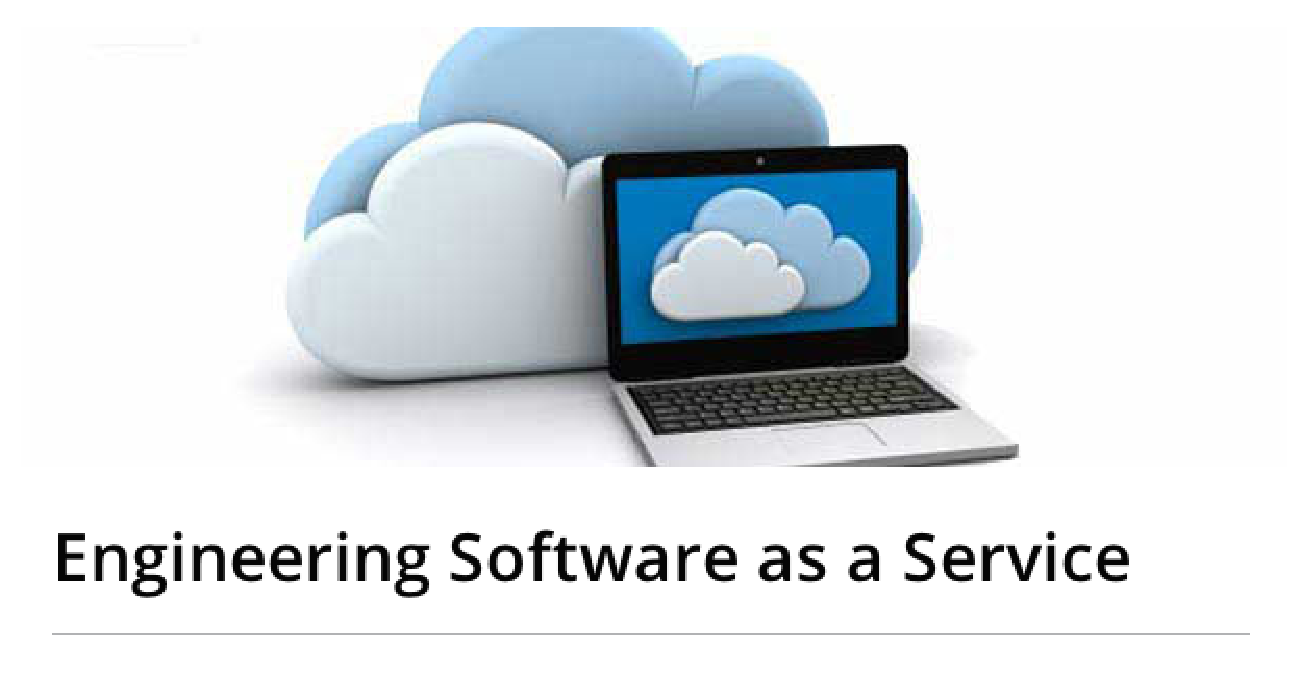
\includegraphics[width=0.4\textwidth]{img/sassmoc.eps}
  \end{center}
  \framebreak
  %+++++++++++++++++++++++++++++++++++++++++++++++++++++++++++++++++++++++++++++++++++++++++++++++++++++++++++++++++++++++++++++++++++++++++++
  
  \begin{itemize}
    \item Este DSL se consideró idóneo para comenzar con la elaboración de este TFG:
    \begin{itemize}
      \item A partir de un fichero Ruby que recibe como entrada, genera un cuestionario en los formatos anteriormente descritos.
    \end{itemize}
    
    \begin{center}
      \fbox{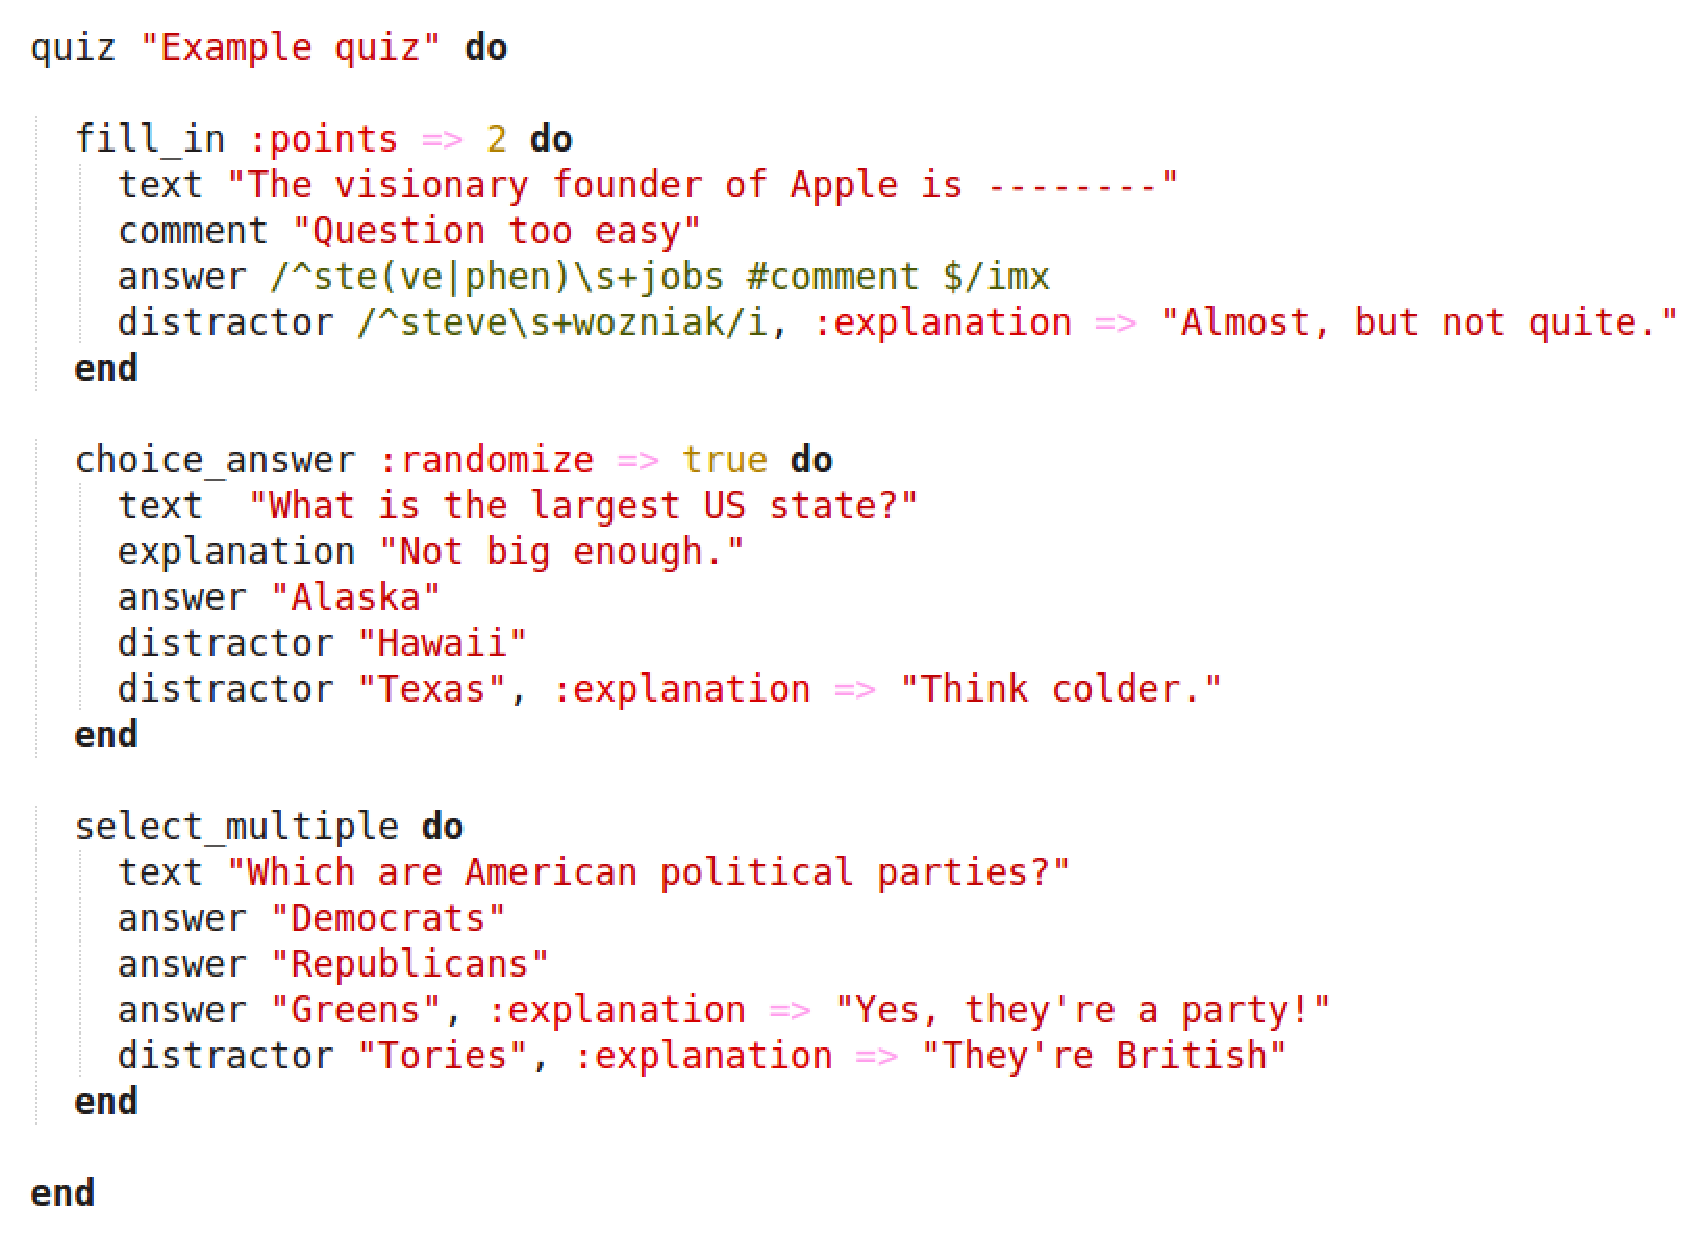
\includegraphics[width=0.65\textwidth]{img/quiz.eps}}
    \end{center}
    
    \framebreak
    %+++++++++++++++++++++++++++++++++++++++++++++++++++++++++++++++++++++++++++++++++++++++++++++++++++++++++++++++++++++++++++++++++++++++++++
    
    {\bfseries {\Large Funcionamiento}}
    \bigskip
    \bigskip
    
      \begin{columns}
        % First column
        \begin{column}{3cm}
          
\includegraphics[width=0.7\textwidth]{img/ruby_file.eps} \\
          \hspace*{0.1cm}
          example.rb
        \end{column}
        % Second column
        \begin{column}{0.1px}
          $\rightarrow$
        \end{column}
        % Third column
        \begin{column}{4cm}
          \hspace*{0.8cm}
          \begin{center}
            
\includegraphics[width=0.6\textwidth]{img/terminal_icon.eps} \\
          \end{center}
          \tiny{\textit{[\textasciitilde]\$ ruql example.rb Html5 \textgreater \,output.html}}
        \end{column}
        % Fourth column
        \begin{column}{0.5cm}
          $\rightarrow$
        \end{column}
        % Fifth column
        \begin{column}{3cm}
          
\includegraphics[width=0.7\textwidth]{img/file_html.eps} \\
          output.html
        \end{column}
      \end{columns}
    
    \framebreak
    %+++++++++++++++++++++++++++++++++++++++++++++++++++++++++++++++++++++++++++++++++++++++++++++++++++++++++++++++++++++++++++++++++++++++++++
    
    \item Entablé contacto con Armando comentándole lo que se pretendía hacer y
    accedió de amablemente a incorporar mis cambios a su gema original. 
    \item Actualmente soy {\bfseries colaborador} en su repositorio.
    \hspace*{0.8cm} 
    
\includegraphics[width=0.1\textwidth]{img/like.eps}
  \end{itemize}
\end{frame}
  %+++++++++++++++++++++++++++++++++++++++++++++++++++++++++++++++++++++++++++++++++++++++++++++++++++++++++++++++++++++++++++++++++++++++++++
  
\section{Trabajos Relacionados y Perfil de Usuario}
\begin{frame}[allowframebreaks]
  \frametitle{Trabajos Relacionados y Perfil de Usuario}
  
  \begin{itemize}
    \item Existen numerosas plataformas que permiten realizar cuestionarios y calificar a los alumnos, como por ejemplo {\bfseries Moodle}.
    \begin{center}
      
\includegraphics[width=0.35\textwidth]{img/moodle.eps}
    \end{center}
    Sin embargo, no cuenta con la posibilidad de añadir preguntas propias de las ramas de \textit{Ingeniería}, como pueden ser aquellas
    cuyas respuestas son evaluadas por programas escritos por el profesor.
    \framebreak
    %+++++++++++++++++++++++++++++++++++++++++++++++++++++++++++++++++++++++++++++++++++++++++++++++++++++++++++++++++++++++++++++++++++++++++++ 
    
    \item La herramienta propuesta está principalmente orientada hacia un perfil de profesor concreto:
    \begin{itemize}
      \item Docente de alguna rama de Ingeniería.
      \item Con conocimientos avanzados de programación y administración de sistemas.
    \end{itemize}
    
    \begin{center}
      
\includegraphics[width=0.5\textwidth]{img/meme.eps}
    \end{center}
  \end{itemize}
  
\end{frame}
%++++++++++++++++++++++++++++++++++++++++++++++++++++++++++++++++++++++++++++++  

\section{Objetivos}
\begin{frame}
  \frametitle{Objetivos}
  
  Los objetivos que se han propuesto a completar han sido los siguientes:
  \begin{columns}
    % First column
    \begin{column}{9cm}
      \begin{itemize}
        \item Revisión biliográfica y consulta del estado del arte.
        \item Extensión del DSL para la elaboración de cuestionarios de modo que permita:
        \begin{itemize}
          \item Nuevos tipos de preguntas como, por ejemplo, de código.
          \item Generar cuestionarios autoevaluables para entrenamiento del alumnado en formato HTML.
          \item Generar una aplicación Web autocorrectora de cuestionarios.
        \end{itemize}
      \end{itemize}
    \end{column}
    % Second column
    \begin{column}{5cm}
      
\includegraphics[width=0.7\textwidth]{img/checklist.eps}
    \end{column}
  \end{columns}
  
\end{frame}

%++++++++++++++++++++++++++++++++++++++++++++++++++++++++++++++++++++++++++++++  

\section{Tecnología usada}
\begin{frame}
  \frametitle{Tecnología usada}
  
  
\includegraphics[width=0.1\textwidth]{img/ruby.eps}
  \hspace*{1.2cm}
  
\includegraphics[width=0.13\textwidth]{img/HTML5.eps}
  \hspace*{1.2cm}
  
\includegraphics[width=0.1\textwidth]{img/css3.eps}
  \hspace*{1.2cm}
  
\includegraphics[width=0.1\textwidth]{img/js.eps}
  \hspace*{1.2cm}
  
\includegraphics[width=0.13\textwidth]{img/bootstrap.eps}
  \newline
  \newline
  
\includegraphics[width=0.25\textwidth]{img/jquery.eps}
  \hspace*{1.2cm}
  
\includegraphics[width=0.25\textwidth]{img/xregexp.eps}
  \hspace*{1.2cm}
  
\includegraphics[width=0.25\textwidth]{img/mathjax.eps}
  \newline
  \newline
  
\includegraphics[width=0.15\textwidth]{img/codemirror.eps}
  \hspace*{1.2cm}
  
\includegraphics[width=0.15\textwidth]{img/mocha.eps}
  \hspace*{1.2cm}
  
\includegraphics[width=0.15\textwidth]{img/chai.eps}
  \hspace*{1.2cm}
  
\includegraphics[width=0.15\textwidth]{img/karma.eps}
  \newline
  \newline
  
\includegraphics[width=0.15\textwidth]{img/sinatra.eps}
  \hspace*{1.0cm}
  
\includegraphics[width=0.15\textwidth]{img/github.eps}
  \hspace*{1.0cm}
  
\includegraphics[width=0.12\textwidth]{img/heroku.eps}
  \hspace*{1.0cm}
  
\includegraphics[width=0.12\textwidth]{img/oauth.eps}
  \hspace*{1.0cm}
  \includegraphics[width=0.13\textwidth]{img/google_drive.eps}
\end{frame}

%++++++++++++++++++++++++++++++++++++++++++++++++++++++++++++++++++++++++++++++  

\section{Metodología de desarrollo}
\begin{frame}
  \frametitle{Metodología de desarrollo}
  
  Metodología {\bfseries ágil}:
  \begin{itemize}
    \item Reuniones semanales estableciendo iteraciones cortas.
    \item Desarrollo, testing y presentación de resultados y prototipos cada semana.
    \item Solución de problemas e incorporación de nuevas características. 
  \end{itemize}
  \bigskip
  
  {\bfseries GitHub}:
  \begin{columns}
    % First column
    \begin{column}{9cm}
      \begin{itemize}
        \item Control de versiones usando \textit{branching}.
        \item Gestión de incidencias y mejoras usando \textit{issues}.
        \item Contacto con Armando para los \textit{Pull Requests}.
      \end{itemize}
    \end{column}
    % Second column
    \begin{column}{4cm}
      \begin{figure}
        
\includegraphics[width=0.7\textwidth]{img/octocat.eps}
      \end{figure}
    \end{column}
  \end{columns}
\end{frame}

%++++++++++++++++++++++++++++++++++++++++++++++++++++++++++++++++++++++++++++++

\section{Resultados}
\begin{frame}
\frametitle{Resultados}
  
  \begin{center}
    \Huge{Resultados}
  \end{center}
\end{frame}

\subsection{Corrección de errores y mejoras de la gema original}
\begin{frame}
\frametitle{Corrección de errores y mejoras de la gema original}
  \bigskip
  \bigskip
  
  \begin{itemize}
    \item Corrección de errores de funcionamiento de la gema.
    \item Corrección de tests.
    \item Refactorización de código.
    \item Añadido manejo de excepciones y mejora de los mensajes de error.
  \end{itemize}
  
  \begin{figure}
    \hfill\includegraphics[width=0.2\textwidth]{img/tick.eps}
  \end{figure}
  
\end{frame}
  %+++++++++++++++++++++++++++++++++++++++++++++++++++++++++++++++++++++++++++++++++++++++++++++++++++++++++
  
\subsection{Cuestionarios de entrenamiento para alumnos: HtmlForm renderer}
  
\begin{frame}[allowframebreaks]
\frametitle{Cuestionarios de entrenamiento para alumnos: HtmlForm renderer}
  Se genera un fichero HTML que contiene un formulario web. 
  \bigskip
  
  Características destacadas:
  \begin{itemize}
    \item Validación por {\bfseries JavaScript}.
    \item {\bfseries Local Storage} de HTML5 para almacenar las respuestas introducidas.
    \item Expresiones regulares más potentes usando 
\includegraphics[width=0.23\textwidth]{img/xregexp.eps}
    \framebreak
    %+++++++++++++++++++++++++++++++++++++++++++++++++++++++++++++++++++++++++++++++++++++++++
    
    \item Soporte a preguntas de completar que evalúan código JavaScript.
    \bigskip
    \begin{center}
      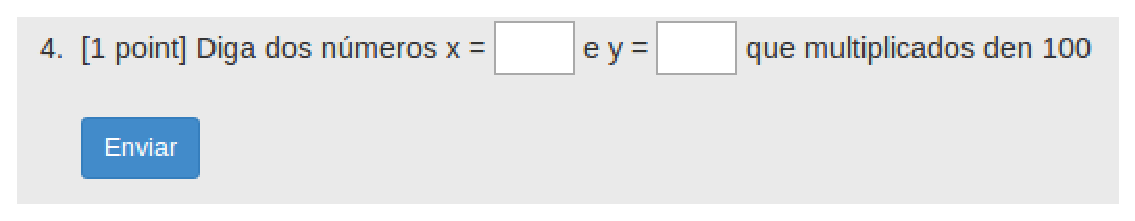
\includegraphics[width=0.8\textwidth]{img/fi_p.eps}
    \end{center}
    \bigskip
    
    \item Soporte a expresiones escritas en {\bfseries LaTeX} usando {\bfseries MathJax}.
    \bigskip
    \begin{center}
      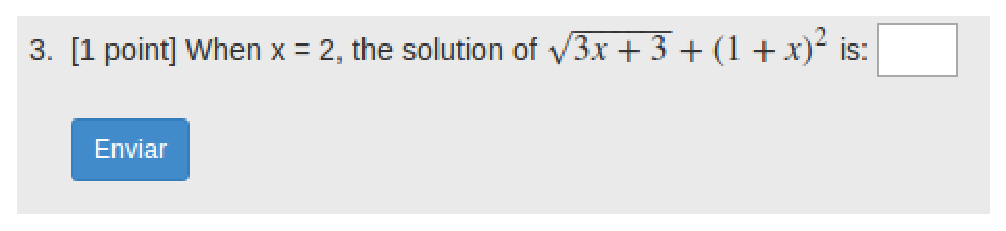
\includegraphics[width=0.8\textwidth]{img/latex.eps}
    \end{center}
    \framebreak
    %+++++++++++++++++++++++++++++++++++++++++++++++++++++++++++++++++++++++++++++++++++++++++
    
    \item Soporte a preguntas de programación (código JavaScript).
    \bigskip
    \begin{center}
      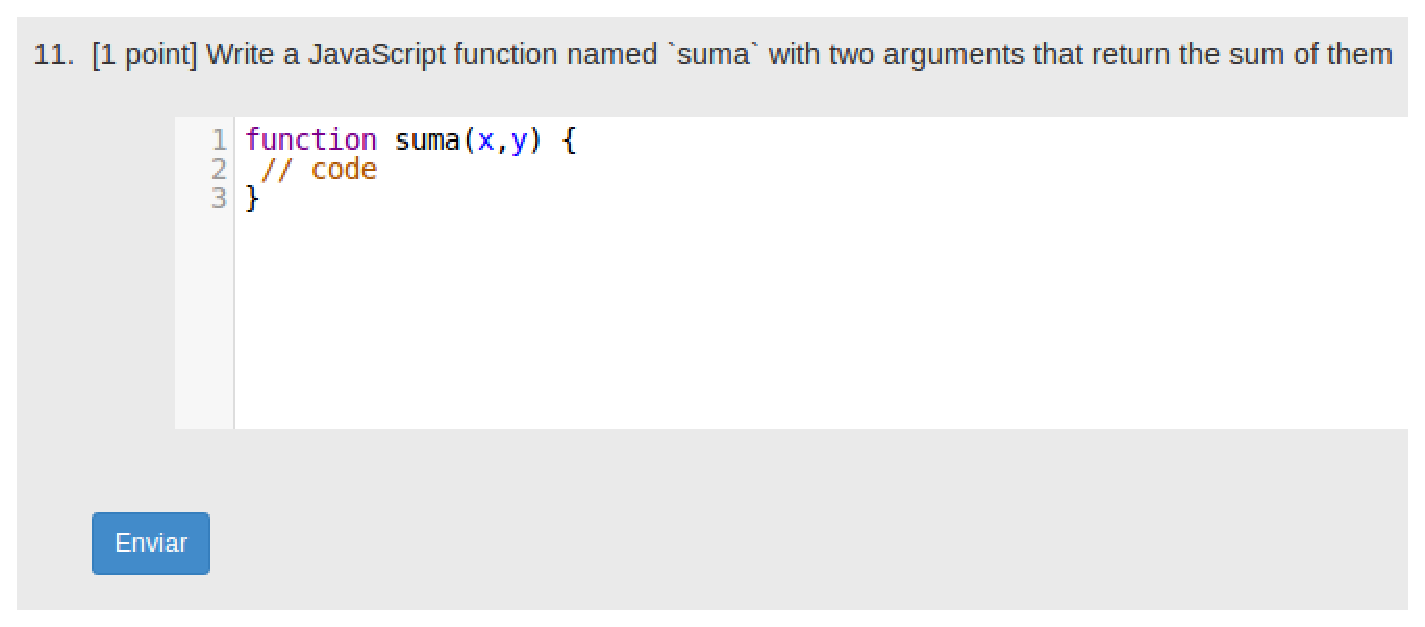
\includegraphics[width=0.9\textwidth]{img/programming.eps}
    \end{center}
    \framebreak
    %+++++++++++++++++++++++++++++++++++++++++++++++++++++++++++++++++++++++++++++++++++++++++
    
    \item Soporte a preguntas de Drag and Drop.
    \bigskip
    \begin{columns}
      % First column
      \begin{column}{7cm}
        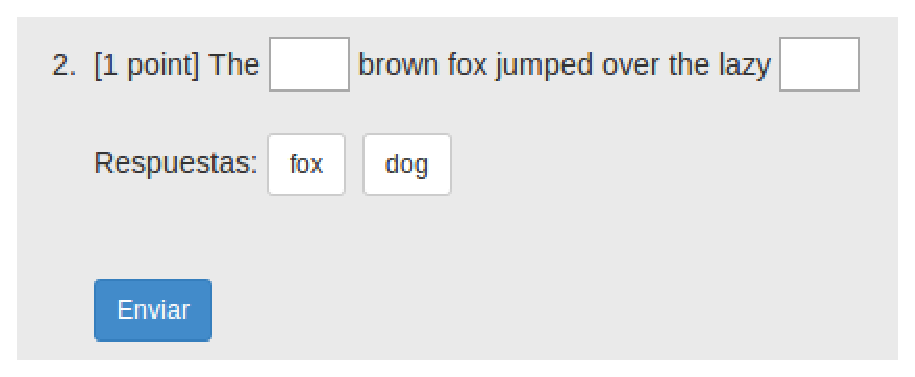
\includegraphics[width=0.9\textwidth]{img/ddfi.eps}
        \newline
        \newline
        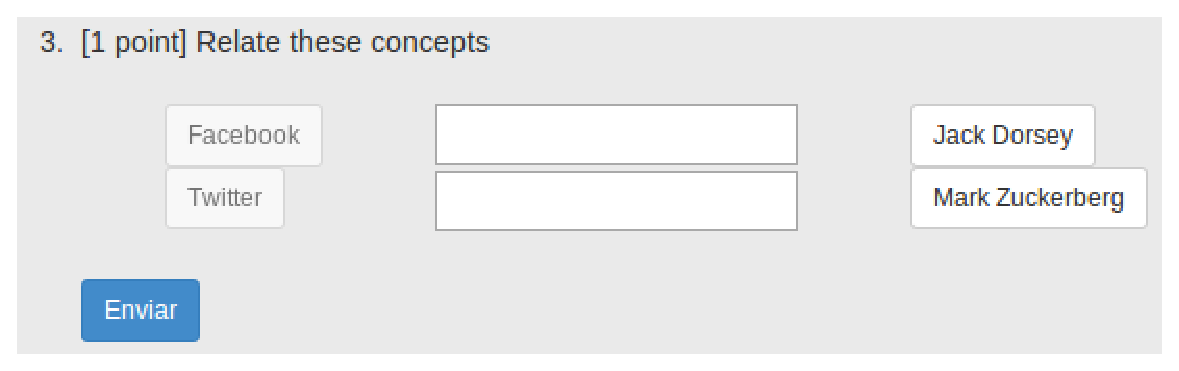
\includegraphics[width=0.9\textwidth]{img/ddmc.eps}
      \end{column}
      % Second column
      \begin{column}{5.5cm}
        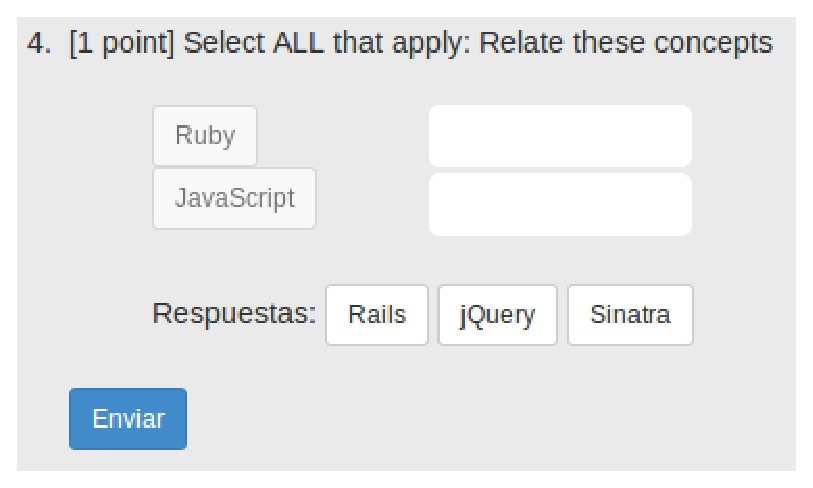
\includegraphics[width=1\textwidth]{img/ddsm.eps}
      \end{column}
    \end{columns}
    \framebreak
    %+++++++++++++++++++++++++++++++++++++++++++++++++++++++++++++++++++++++++++++++++++++++++
    
    \item Posibilidad de mostrar las respuestas correctas
    \bigskip
    \begin{itemize}
      \item Mediante menú contextual:
      \begin{center}
        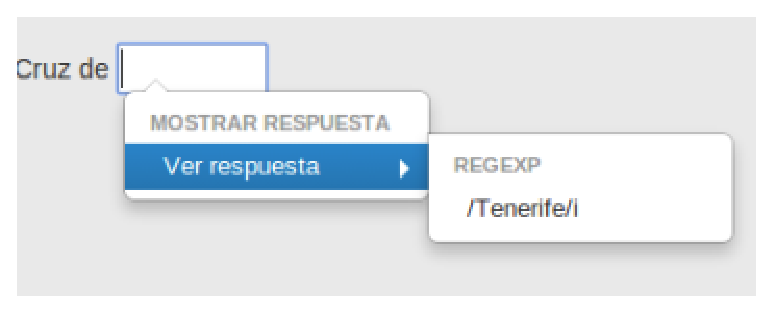
\includegraphics[width=0.5\textwidth]{img/show_answer.eps}
      \end{center}
      \item Mediante botones:
      \begin{center}
        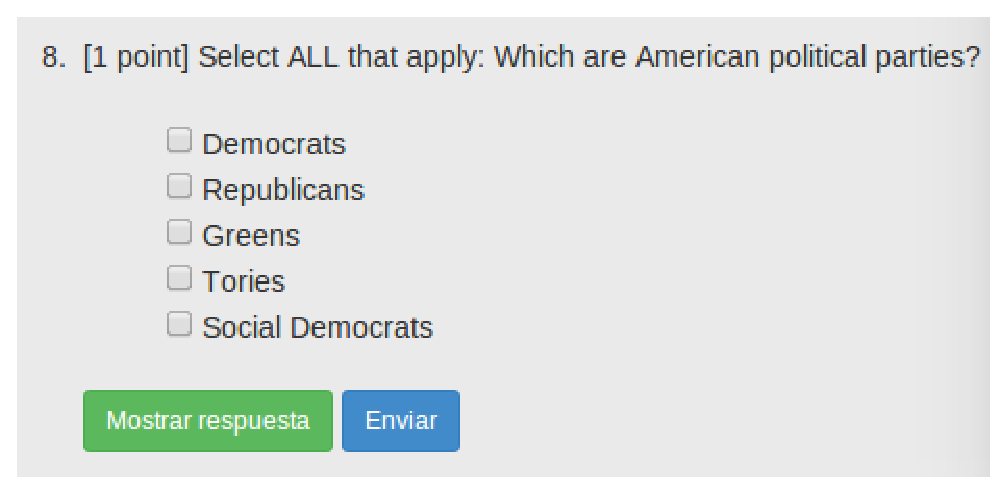
\includegraphics[width=0.5\textwidth]{img/sm.eps}
      \end{center}  
    \end{itemize}
    
  \end{itemize}
  \framebreak
  %+++++++++++++++++++++++++++++++++++++++++++++++++++++++++++++++++++++++++++++++++++++++++
  
  {\bfseries {\Large Funcionamiento}}
  \bigskip  
  \bigskip
  
  \begin{columns}
    % First column
    \begin{column}{3cm}
      
\includegraphics[width=0.7\textwidth]{img/ruby_file.eps} \\
      \hspace*{0.1cm}
      example.rb
    \end{column}
    % Second column
    \begin{column}{0.1px}
      $\rightarrow$
    \end{column}
    % Third column
    \begin{column}{5cm}
      \hspace*{0.8cm}
      \begin{center}
        
\includegraphics[width=0.55\textwidth]{img/terminal_icon.eps} \\
        \tiny{\textit{[\textasciitilde]\$ ruql example.rb HtmlForm \textgreater \,output.html}}
      \end{center}
    \end{column}
    % Fourth column
    \begin{column}{0.5cm}
      $\rightarrow$
    \end{column}
    % Fifth column
    \begin{column}{3cm}
      
\includegraphics[width=0.7\textwidth]{img/file_html.eps} \\
      output.html
    \end{column}
  \end{columns}
  
\end{frame}
  %+++++++++++++++++++++++++++++++++++++++++++++++++++++++++++++++++++++++++++++++++++++++++++++++++++++++++++
  
\subsection{Aplicación correctora de exámenes: Sinatra renderer}

\begin{frame}[allowframebreaks]
\frametitle{Aplicación correctora de exámenes: Sinatra renderer}
  Genera una aplicación Sinatra con todo lo necesario para ser desplegada.
  \bigskip
  
  Características:
  \begin{itemize}
    \item Roles de usuarios: profesores y alumnos.
    \item Autenticación usando {\bfseries OAuth} con las cuentas de Gmail.
    \item Ventana temporal en la que el cuestionario estará disponible.
    \item Corrección de los cuestionarios realizados por los alumnos.
    \item Soporte a los tipos de preguntas explicados anteriormente.
    \item Soporte a preguntas de programación (código en {\bfseries Ruby}).
    \framebreak
    %+++++++++++++++++++++++++++++++++++++++++++++++++++++++++++++++++++++++++++++++++++++++++++++++++++++++++++
    
    \begin{center}
      {\bfseries {\Large Funcionamiento}}
    \end{center}
    
    \begin{columns}
      % First column
      \begin{column}{3.05cm}
        \hspace*{0.3cm}
        
\includegraphics[width=0.5\textwidth]{img/ruby_file.eps} \\
        \hspace*{0.3cm}
        example.rb
        \newline
        \newline
        \hspace*{0.3cm}
        
\includegraphics[width=0.5\textwidth]{img/yml_file.eps} \\
        \hspace*{0.3cm}
        config.yml
        \newline
        \newline
        \hspace*{0.3cm}
        
\includegraphics[width=0.5\textwidth]{img/csv_file.eps} \\
        \hspace*{0.3cm}
        students.csv
      \end{column}
      % Second column
      \begin{column}{0.1px}
        $\rightarrow$
      \end{column}
      % Third column
      \begin{column}{4cm}
        \hspace*{0.8cm}
        \begin{center}
          
\includegraphics[width=0.6\textwidth]{img/terminal_icon.eps} \\
          \tiny{\textit{[\textasciitilde]\$ ruql example.rb Sinatra}}
        \end{center}
      \end{column}
      % Fourth column
      \begin{column}{0.5cm}
        $\rightarrow$
      \end{column}
      % Fifth column
      \begin{column}{4cm}
        \begin{center}
          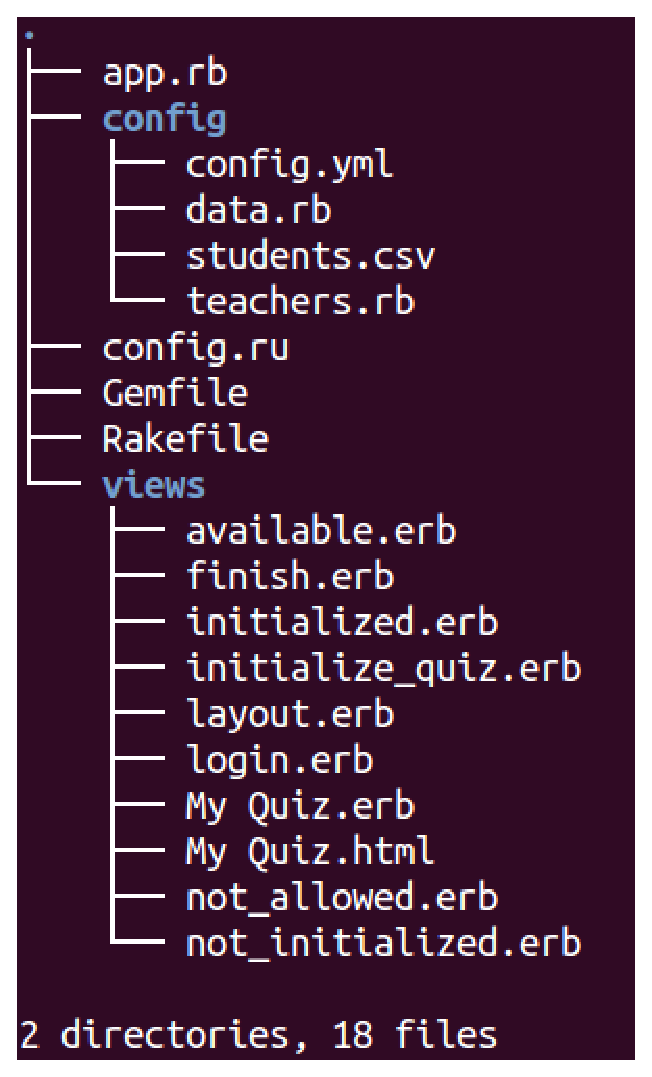
\includegraphics[width=0.9\textwidth]{img/tree.eps}
        \end{center}
      \end{column}
    \end{columns}
    
    \framebreak
    %+++++++++++++++++++++++++++++++++++++++++++++++++++++++++++++++++++++++++++++++++++++++++++++++++++++++++++
    
    \begin{columns}[tc]
      % First column
      \begin{column}{7cm}
        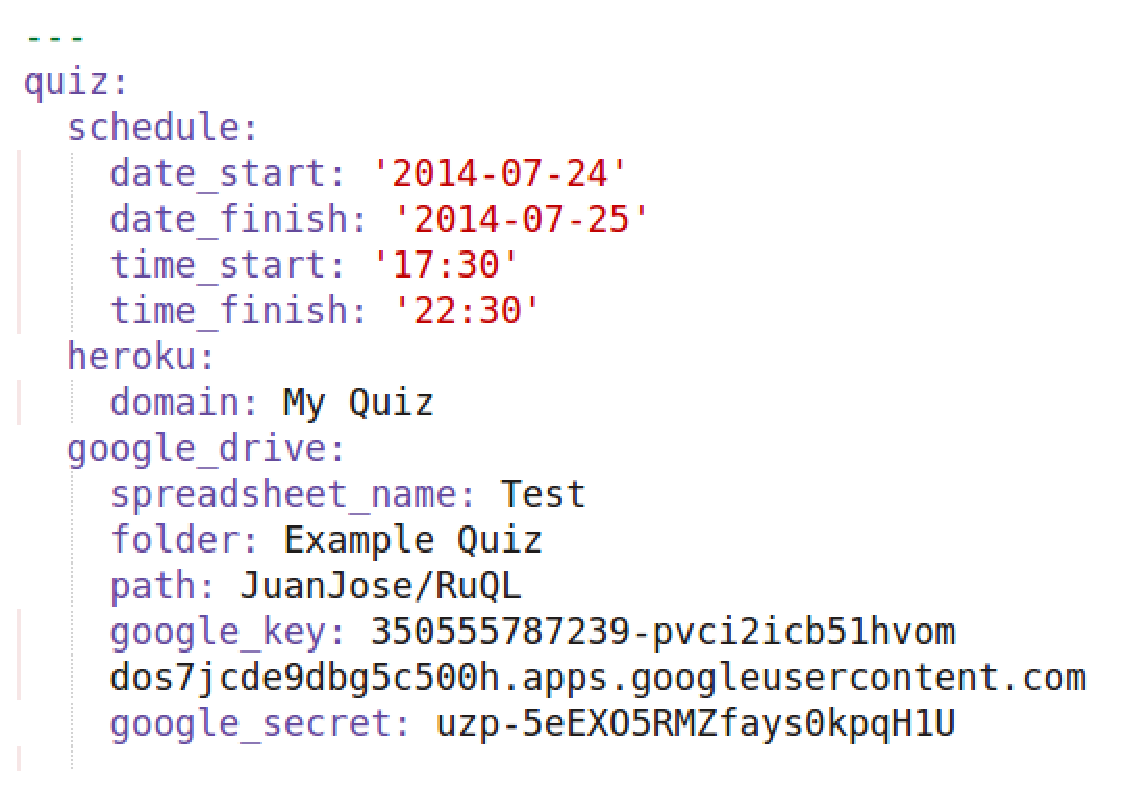
\includegraphics[width=1\textwidth]{img/yml.eps} \\
        \hspace*{1cm}
        config.yml
      \end{column}
      % Second column
      \begin{column}{5cm}
        \includegraphics[width=1\textwidth]{img/quiz_sinatra.eps} \\
        \hspace*{1cm}
        example.rb
      \end{column}
    \end{columns}
    \bigskip
    
    \begin{center}
      \includegraphics[width=0.7\textwidth]{img/csv.eps} \\
      students.csv
    \end{center}
    
    \framebreak
    %+++++++++++++++++++++++++++++++++++++++++++++++++++++++++++++++++++++++++++++++++++++++++++++++++++++++++++
    
    \item Almacenamiento del cuestionario, respuestas y notas de los alumnos en {\bfseries Google Drive}.
    \bigskip
    \begin{center}
      \includegraphics[width=0.9\textwidth]{img/app0.eps}
      \newline
      \newline
      \includegraphics[width=0.5\textwidth]{img/app6.eps}
    \end{center}
    
    \framebreak
    %+++++++++++++++++++++++++++++++++++++++++++++++++++++++++++++++++++++++++++++++++++++++++++++++++++++++++++
    
    \begin{center}
      \includegraphics[width=0.8\textwidth]{img/app3.eps}
    \end{center}
    \framebreak
    %+++++++++++++++++++++++++++++++++++++++++++++++++++++++++++++++++++++++++++++++++++++++++++++++++++++++++++
    
    \begin{center}
      \includegraphics[width=0.6\textwidth]{img/app4.eps}
    \end{center}
    \framebreak
    %+++++++++++++++++++++++++++++++++++++++++++++++++++++++++++++++++++++++++++++++++++++++++++++++++++++++++++
    
    \begin{center}
      \includegraphics[width=0.9\textwidth]{img/app1.eps} \\
      \bigskip
      \begin{columns}
        \begin{column}{4cm}
          \includegraphics[width=1.2\textwidth]{img/app2.eps}
        \end{column}
        \begin{column}{4cm}
          \includegraphics[width=1.1\textwidth]{img/app7.eps}
        \end{column}
      \end{columns}
    \end{center}
    \framebreak
    %+++++++++++++++++++++++++++++++++++++++++++++++++++++++++++++++++++++++++++++++++++++++++++++++++++++++++++
    
    \begin{center}
      \includegraphics[width=0.5\textwidth]{img/app5.eps}
    \end{center}
    
  \end{itemize}
\end{frame}
%++++++++++++++++++++++++++++++++++++++++++++++++++++++++++++++++++++++++++++++  

\section{Conclusiones y Trabajos Futuros/Conclusions and Future Work}
\begin{frame}[allowframebreaks]
  \frametitle{Conclusiones y Trabajos Futuros/Conclusions and Future Work}
  
  \begin{itemize}
    \item Esta herramienta pretende ser un complemento para plataformas como Moodle al ofrecer la posibilidad de
    especificar preguntas de programación.
    \item Ofrece una solución innovadora para el almacenamiento de los datos de los exámenes: {\bfseries Google Drive}.
    Permite gestionar de forma más cómoda los datos generados en lugar de usar bases de datos.
    \item Por otra parte, considerando aspectos éticos y de seguridad, se hace uso de {\bfseries OAuth} para la autentificación de usuarios con el fin de evitar
    posibles problemas de phishing y exposición de datos sensibles a terceras personas.
  \end{itemize}
  \framebreak
  %+++++++++++++++++++++++++++++++++++++++++++++++++++++++++++++++++++++++++++++++++++++++++++++++++++++++++++++++++++++++++++++++++++++++++++
  
  {\bf Trabajos Futuros:}
  \begin{itemize}
    \item Resolver los problemas de seguridad relacionados con evaluar el código escrito de los alumnos.
    \item Dar soporte a preguntas con respuestas de código en otros lenguajes de programación.
    \item Ofrecer una alternativa de despliegue distinta a Heroku.
    \item Escribir \textit{renderers} para dar soporte a otros formatos usados por diversas plataformas educativas (Ej: MoodleXML, Gift, etc.).
  \end{itemize}
  \framebreak
  %+++++++++++++++++++++++++++++++++++++++++++++++++++++++++++++++++++++++++++++++++++++++++++++++++++++++++++++++++++++++++++++++++++++++++++
  
  \begin{itemize}
    \item This tool intends to complement learning management systems with new capabilities like the possibility to specify {\bfseries programming questions}.
    \item It uses {\bfseries Google Drive} for the storage of exams data (instead using databases),
    providing in this way a more natural solution from the lecturer perspective.
    \item On the other hand, keeping in mind ethic and legal topics, we use {\bfseries OAuth} to delegate the authentication to Google. 
    This way, we avoid security bugs as the phishing or the exposure of sensitive information to third people.
  \end{itemize}
  \framebreak
  %+++++++++++++++++++++++++++++++++++++++++++++++++++++++++++++++++++++++++++++++++++++++++++++++++++++++++++++++++++++++++++++++++++++++++++
  
  {\bf Future Work:}
  \begin{itemize}
    \item Solve the security problem related with the evaluation of student code in the server.
    \item Provide support to questions with answers written in other programming languages.
    \item Provide a deployment alternative different to Heroku.
    \item To write renderers giving support to other formats (MoodleXML, Gift, etc.) used by a variety of learning platforms.
  \end{itemize}
\end{frame}

%++++++++++++++++++++++++++++++++++++++++++++++++++++++++++++++++++++++++++++++ 

\section{Bibliografía}
\begin{frame}[allowframebreaks]
  \frametitle{Bibliografía}
  \bibliographystyle{ieeetr}
  \bibliography{presentacion_tfg}
  \nocite{*}
\end{frame}

\begin{frame}
  \frametitle{Fin de la presentación}
  \begin{center}
    \Huge{Gracias por su atención}
  \end{center}
\end{frame}

\end{document}
